\documentclass [a4paper] {article}
\usepackage[utf8]{inputenc}
\title{Ciencia de datos, práctica 4}
\author{Juan Casado Ballesteros, Samuel García Gonzalez, Iván Anaya Martín}
\usepackage{Sweave}
\begin{document}
\maketitle

\begin{abstract}
A lo largo de esta práctica analizaremos y compararemos distintos métodos de clasificación no supervisada o clusterización.

Utilizaremos el algoritmo de k-mean para realizar el ejercicio propuesto y la primera parte del ejercicio libre.
Nos centraremos principalmente en las técnicas de selección del número de clusters óptimo para lo cual exploraremos tres de ellas.
Adicionalmente hemos relizado una implementación propia de k-means que validaremos comparándola con los resultados de la implementación de R.
La ventaja de nuestra implementación frente a la de R es que nos permite visualizar paso a paso el estado de cada iteración del algoritmo.
Esto nos permite ver cómo se desplazan los centroides así como ver en cada momento la clasificación actual de los elementos de la muestra.

En la segunda parte del ejercicio libre utilizaremos los algoritmos de clasificación jerárquica aglomerativo y divisivo.
En el algoritmo aglomerativo partimos de que cada elemento de la muestra es una clases.
En cada iteración elegiremos las dos clases más próximas y la uniremos en una nueva clase creando así una estructura de árbol.
En el algoritmo divisivo todos los elementos serán consderados una única clase al inicio de la ejecución.
En cada iteración separaremos la clase en dos pudiendo contener cada una de ellas uno o más elementos creando así una estructura de árbol.
Las principales variaciones en estos métodos residen en la métrica utilizada para calcular la distancia entre clases a partir de la cual decidimos cuando separarlas o unirlas.
Exploraremos distintas métricas, visualizaremos los árboles generados y compararemos las clasificaciones jerárquicas entre si y con los resultados de k-means.

Debido a que deseamos comparar los resultados de k-means con la clasificación jerarquica utilizaremos para explorar ambos algoritmos el mismo dataset.
Se utilizará un dataset obtenido de kaggle en que se presentan las características de un conjunto de semillas.
\end{abstract}

\newpage
\tableofcontents


\newpage
\section{K-means sobre la muestra proporcionada}

Aplicaremos el algoritmo k-means sobre la muestra que se nos proporciona.
Este algoritmo clasificará de forma no supervisada la muestra en tantas clases como indiquemos.
En primer lugar deberemos cargar esta desde un archivo .txt.
\begin{Schunk}
\begin{Sinput}
> datos1 <- read.table("datos1.txt")
> datos1
\end{Sinput}
\begin{Soutput}
  Teoria Laboratorio
1      4           4
2      3           5
3      1           2
4      5           5
5      0           1
6      2           2
7      4           5
8      2           1
\end{Soutput}
\end{Schunk}

Para esta muestra tal y como podemos ver y tal y como vimos en clase el número adecuado de centroides es 2.
Ubicaremos dos puntos a partir de los cuales se ejecutará el algoritmo.
\begin{Schunk}
\begin{Sinput}
> centroides <- matrix(c(0,1,2,2),2,2)
> centroides <- t(centroides)
> centroides
\end{Sinput}
\begin{Soutput}
     [,1] [,2]
[1,]    0    1
[2,]    2    2
\end{Soutput}
\end{Schunk}

Realizamos la ejecución del algoritmo con la implementación que R nos proporciona.
\begin{Schunk}
\begin{Sinput}
> classkms<-kmeans(datos1,centroides,4)
\end{Sinput}
\end{Schunk}

\subsection{Evaluación de la solución obtenida}
Podemos ver a que clase pertenecen cada uno de los elementos de la muestra.
Nuestra muestra tiene un total de ocho elementos que se han clasificado en dos clases (clase 1 y clase 2).
\begin{Schunk}
\begin{Sinput}
> classkms$cluster
\end{Sinput}
\begin{Soutput}
1 2 3 4 5 6 7 8 
2 2 1 2 1 1 2 1 
\end{Soutput}
\end{Schunk}
Centroides de cada una de las dos clases.
Son los puntos que minimizan las distancias a los elementos de la muestra, desde ellos a los elementos de su clase.
\begin{Schunk}
\begin{Sinput}
> classkms$centers
\end{Sinput}
\begin{Soutput}
  Teoria Laboratorio
1   1.25        1.50
2   4.00        4.75
\end{Soutput}
\end{Schunk}
Cantidad de elementos que pertenecen a cada una de las clases obtenidas.
\begin{Schunk}
\begin{Sinput}
> classkms$size
\end{Sinput}
\begin{Soutput}
[1] 4 4
\end{Soutput}
\end{Schunk}
Iteraciones necesarias para realizar la clasificación. Este valor no se refiere a las iteraciones del algoritmo,
con una sola iteración no se hubiera podido llegar a la solución.
\begin{Schunk}
\begin{Sinput}
> classkms$iter
\end{Sinput}
\begin{Soutput}
[1] 1
\end{Soutput}
\end{Schunk}
Indica si la clasificación obtenida es válida o no.
K-means con unos centroides iniciales mal-intencionadamente elegidos puede no llegar a una solución válida
\begin{Schunk}
\begin{Sinput}
> classkms$ifault
\end{Sinput}
\begin{Soutput}
[1] 0
\end{Soutput}
\end{Schunk}
Distancia cuadrática media entre los centroides, deseamos que este valor sea alto ya que querríamos que nuestros clusters fueran heterogéneos y bien diferenciados.
\begin{Schunk}
\begin{Sinput}
> classkms$betweenss
\end{Sinput}
\begin{Soutput}
[1] 36.25
\end{Soutput}
\end{Schunk}
Distancia cuadrática media dentro de cada cluster, deseamos obtener valores bajos, es decir, dentro de cada cluster los elementos deben estar próximos, deben ser homogéneos.
\begin{Schunk}
\begin{Sinput}
> classkms$withinss
\end{Sinput}
\begin{Soutput}
[1] 3.75 2.75
\end{Soutput}
\end{Schunk}
Suma de todas las distancias cuadráticas medias dentro de los clusters.
\begin{Schunk}
\begin{Sinput}
> classkms$tot.withinss
\end{Sinput}
\begin{Soutput}
[1] 6.5
\end{Soutput}
\end{Schunk}
Suma de todas las distancias cuadráticas medias dentro de los clusters y la distancia cuadrática media entre clusters.
\begin{Schunk}
\begin{Sinput}
> classkms$totss
\end{Sinput}
\begin{Soutput}
[1] 42.75
\end{Soutput}
\end{Schunk}
Estos últimos cuatro valores ayudan a decidir si el algoritmo ha realizado una clasificación correcta o no.

\subsection{Visualización del resultado}
Dividiremos la muestra en las clases que la ejecución nos ha proporcionado.
Dibujaremos dichas clases junto a sus representantes en una gráfica bidimensional.
Primero deberemos separar los elemntos de la muestra según la clasificación btenida.
\begin{Schunk}
\begin{Sinput}
> clusters <- cbind(classkms$cluster,datos1)
> cluster1 <- subset(clusters,clusters[,1]==1)
> cluster2 <- subset(clusters,clusters[,1]==2)
> cluster1 <- cluster1[,-1]
> cluster2 <- cluster2[,-1]
> clusters <- list(cluster1, cluster2)
\end{Sinput}
\end{Schunk}

Como podemos ver la clasificación se ha realizado correctamente.
\begin{center}
\includegraphics{entrega-representacion_del_resultado}
\end{center}

\subsection{Pasos de la clasificación}
Aunque establezcamos una iteración como número máximo de iteraciones al lanzar el algoritmo este siempre llega a la solución final sin proporcionar los pasos intermedios.
Es por ello que decidimos implementar nuestra propia versión de k-means con la intención de poder mostrar estos pasos intermedios.
A cada iteración del algoritmo extraemos y mostramos el estado de la ejecución en una gráfica distinta.
Podemos ver la evolución de los centroides desde sus posiciones iniciales hasta las finales.
Comprobamos que el resultado de la ejecución con nuestra implementación coincide con el de la implementación de R.
\begin{center}
\begin{Schunk}
\begin{Sinput}
> current_centroides <- centroides
> par(mfrow=c(2,2))
> for (i in 1:4){
+   cluster <- kmeans_cluster (datos1, current_centroides)
+   split <- kmeans_split(datos1, cluster)
+   new_centroides <- kmeans_new_centroids(split)
+   plot_kmeans(split, current_centroides, main=toString(i),
+               xlab="Teroría", ylab="Laboratorio")
+   if (same_centroids(new_centroides, current_centroides)){
+     break
+   }else{
+     current_centroides <- new_centroides
+   }
+ }
> current_centroides
\end{Sinput}
\begin{Soutput}
     [,1] [,2]
[1,] 1.25 1.50
[2,] 4.00 4.75
\end{Soutput}
\end{Schunk}
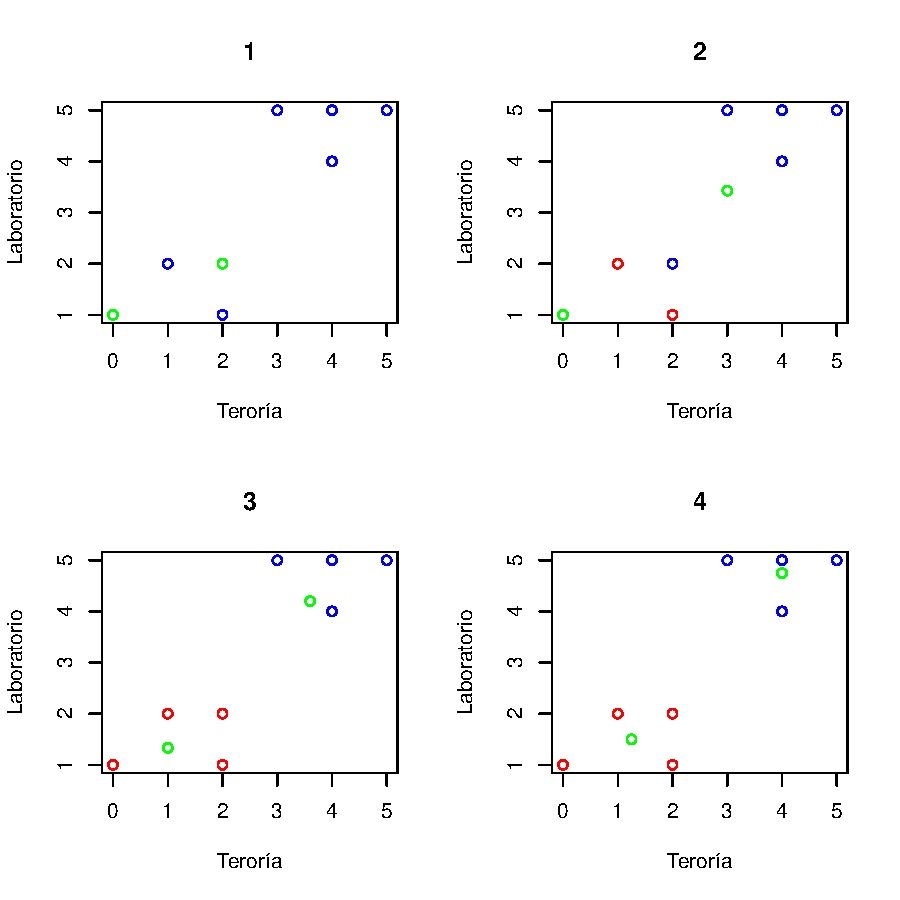
\includegraphics{entrega-custom_kmeans}
\end{center}

\newpage
\section{K-means}
En este apartado vamos a realizar un ejemplo práctico de clustering sobre una muestra obtenida de kaggle.
En dicha muestra se presentan 7 características sobre un conjunto de semillas.

Utilizaremos distintas funciones de las librerías: "tidyverse", "cluster", "factoextra" y "gridExtra" para mostrar los datos y calcular el número óptimo de clusters.
El algoritmo encargado de realizar la clusterización será kmeans del que utilizaremos la implementación que R proporciona.

\subsection{Preparar los datos}
Deberemos eliminar los datos que estén incompletos ya que kmeans no podría manejarlos.
Adicionalmente escalaremos las variables con la intención de hacerlas comparables entre ellas.
Esto es necesario debido a que la escala de las variables de entrada adecta al algoritmo pues se utilizar distancias euclídeas para realizar la clusterización.
Escalar las variables consiste en hacer que la media de cada una de ellas sea 0 y desviación estándar de 1.
Tras haber realizado el escalado aparecerán por tanto valores negativos en las características, estas dejan de estar en sus unidades originales.
\begin{Schunk}
\begin{Sinput}
> df <- read.csv("Seed_Data.csv")
> df <- na.omit(df)
> df <- scale(df)
\end{Sinput}
\end{Schunk}
Mostraramos a continuación un extracto de los datos.
\begin{Schunk}
\begin{Sinput}
> head(df)
\end{Sinput}
\begin{Soutput}
            A            P            C          LK        WK     A_Coef
1  0.14175904  0.214948819 6.045733e-05  0.30349301 0.1413640 -0.9838010
2  0.01116136  0.008204153 4.274938e-01 -0.16822270 0.1969616 -1.7839036
3 -0.19160873 -0.359341919 1.438945e+00 -0.76181710 0.2075516 -0.6658882
4 -0.34626388 -0.474200066 1.036904e+00 -0.68733567 0.3187467 -0.9585276
5  0.44419577  0.329806966 1.371233e+00  0.06650665 0.8032397 -1.5597684
6 -0.16067770 -0.267455401 1.019976e+00 -0.54740087 0.1413640 -0.8235144
         LKG
1 -0.3826631
2 -0.9198156
3 -1.1863572
4 -1.2270506
5 -0.4742231
6 -0.9198156
\end{Soutput}
\end{Schunk}

\newpage
\subsection{Conocer los datos}
Antes de poder realizar cualquier análisis de datos debemos de conocerlos.
En este caso utilizaremos una matriz de distancias para poder hacerlo.
Dicha matriz nos mostrará las distancias entre los elementos que manejamos.
En ella podemos observar que las distancias son heterogéneas entre los elementos, es decir, hay variedad de distancias.
Entre otras cosas la matriz puede ayudarnos a elegir una distancia euclídea para realizar con ella la clasificación seleccionando una que acentúe las desigualdades entre clases.
\begin{center}
\begin{Schunk}
\begin{Sinput}
> dist <- get_dist(df)
> fviz_dist(dist, gradient = list(low = "#00AFBB", mid = "white", high = "#FC4E07"))
\end{Sinput}
\end{Schunk}
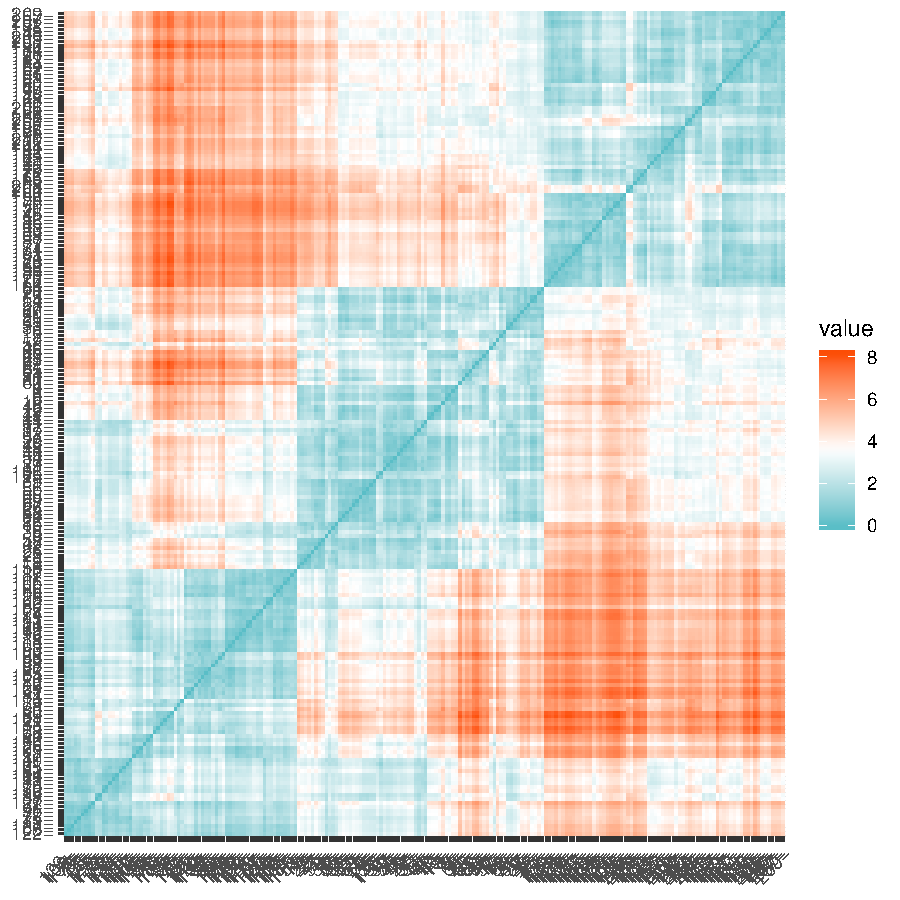
\includegraphics{entrega-kmeans_distances}
\end{center}

\newpage
\subsection{Ejecución del algoritmo}
Ejecutaremos el algoritmo kmeans implementado en R.
En este caso en vez de fijar nosotros los centroides iniciales indicaremos que queremos obtener 2 clases distintas siendo el propio algoritmo quien los establezca.
Adicionalmente indicaremos que queremos probar un total de 25 combinaciones de centroides iniciales.
Dependidendo de las posiciones iniciales obtendremos distintos resultados en la clasificación, ejecuatando el algoritmo varias veces nos aseguramos de quedarnos con una clusterización adecuada.
\begin{Schunk}
\begin{Sinput}
> k2 <- kmeans(df, centers = 2, nstart = 25)
\end{Sinput}
\end{Schunk}
Obtenemos dos centroides, uno para cada clase, además visualizamos la cantidad de elementos en cada una de las clases.
\begin{Schunk}
\begin{Sinput}
> k2$centers
\end{Sinput}
\begin{Soutput}
           A         P          C         LK         WK      A_Coef        LKG
1  1.1379346  1.145151  0.5424726  1.1260130  1.0640703 -0.14617607  1.1468793
2 -0.6588042 -0.662982 -0.3140631 -0.6519023 -0.6160407  0.08462825 -0.6639828
\end{Soutput}
\begin{Sinput}
> k2$size
\end{Sinput}
\begin{Soutput}
[1]  77 133
\end{Soutput}
\end{Schunk}
Adicionalmente mostramos las distancias cuadráticas medias entre los elementos de cada cluster y entre los clusters.
Utilizaremos estas medidas posteriormente para compararlas con la clasificación mediante otros números de clusters.
\begin{Schunk}
\begin{Sinput}
> k2$withinss
\end{Sinput}
\begin{Soutput}
[1] 196.2357 459.7972
\end{Soutput}
\begin{Sinput}
> k2$betweenss
\end{Sinput}
\begin{Soutput}
[1] 806.9672
\end{Soutput}
\end{Schunk}

\newpage
\subsection{Visualización de los resultados}
Tal y como hemos ver en el extrarcto de la muestra cada dato se compone de siete variables.
No obstante solo podemos representar sin realizar alguna simplificación datos tridimensionales.
Es por tanto que la representación no es completamente fiel a la estructura de los datos ya que esta es bidimensional.
La función "fviz cluster" intenta representar los datos lo mejor que puede a partir de las distancias que hay entre los puntos en el espacio de siete dimensiones.
Adicionalmente podremos comprobar más adelante como la función "plot" también se inventa una forma distinta para representar los datos.
Debido a que con "fviz cluster" los datos se ven diferenciados cuanto más lo son los cluster que con "plot" hemos preferido esta primera función para representar los resultados.
Aún así en nuestra implementación propia utilizamos la segunda para poder apreciar las diferencias entre ambos.
\begin{center}
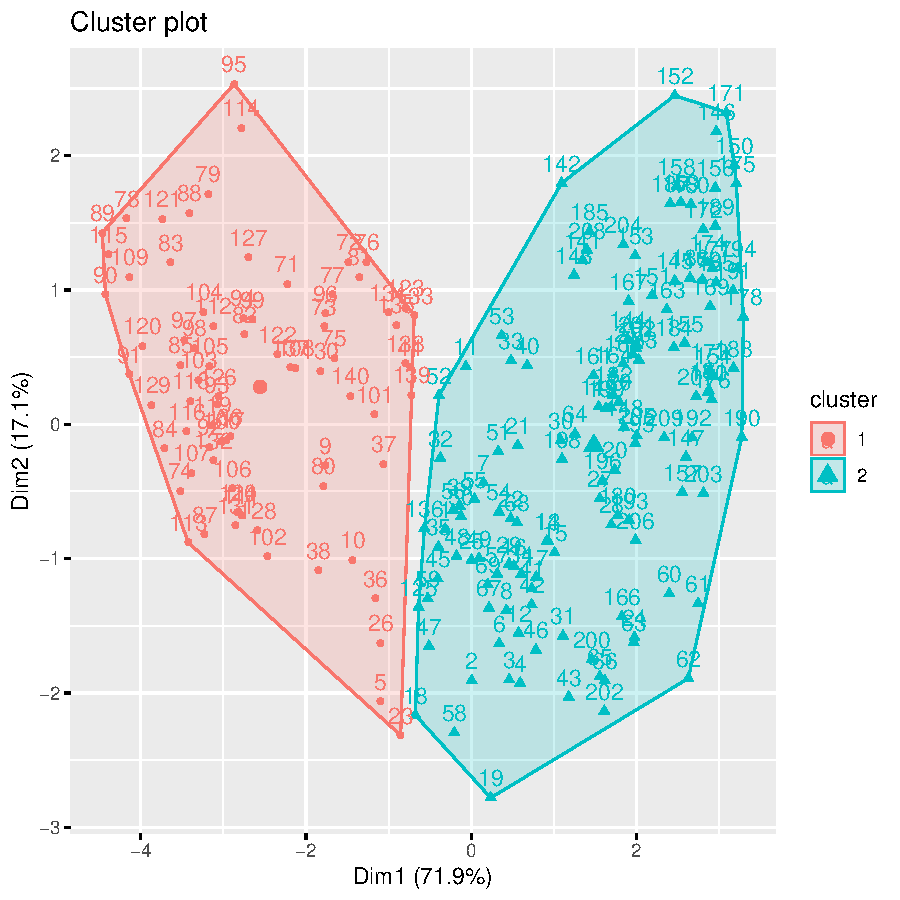
\includegraphics{entrega-kmeans_show_resultse}
\end{center}

\newpage
\subsection{Ejecución con implementación propia}
Realizaremos la misma ejecución utilizando ahora la implementación de kmeans hecha por nosotros.
Para realizar la ejecución tomaremos un vector aleatorio de tantos elementos como el número de clases multiplicado por la cantidad de variables asociadas a cada dato.
Tras la ejecución podremos ver en las gráficas como los centroides logran clasificarse en un número de iteraciones dependiente del vector aleatorio inicial.
Hemos podido observar que el número de iteraciones oscila entre 6 y 9 iteraciones.
Adicionalmente podemos comprobar que los centrides obtenidos con nuestra implementación y con la de R son muy similares.
\begin{center}
\begin{Schunk}
\begin{Sinput}
> datos <- df
> current_centroides <- matrix(runif(14, -2, 2), 2,7)
> par(mfrow=c(3,3))
> for (i in 1:9){
+   cluster <- kmeans_cluster (datos, current_centroides)
+   split <- kmeans_split(datos, cluster)
+   new_centroides <- kmeans_new_centroids(split)
+   plot_kmeans(split, current_centroides, main=toString(i),
+               xlab="Teroría", ylab="Laboratorio")
+   if (same_centroids(new_centroides, current_centroides)){
+     break
+   }else{
+     current_centroides <- new_centroides
+   }
+ }
> current_centroides
\end{Sinput}
\begin{Soutput}
           [,1]       [,2]       [,3]       [,4]       [,5]        [,6]
[1,]  1.1060769  1.1081623  0.5740801  1.0691564  1.0501524 -0.16202391
[2,] -0.6806627 -0.6819461 -0.3532801 -0.6579424 -0.6462476  0.09970702
           [,7]
[1,]  1.0887331
[2,] -0.6699896
\end{Soutput}
\end{Schunk}
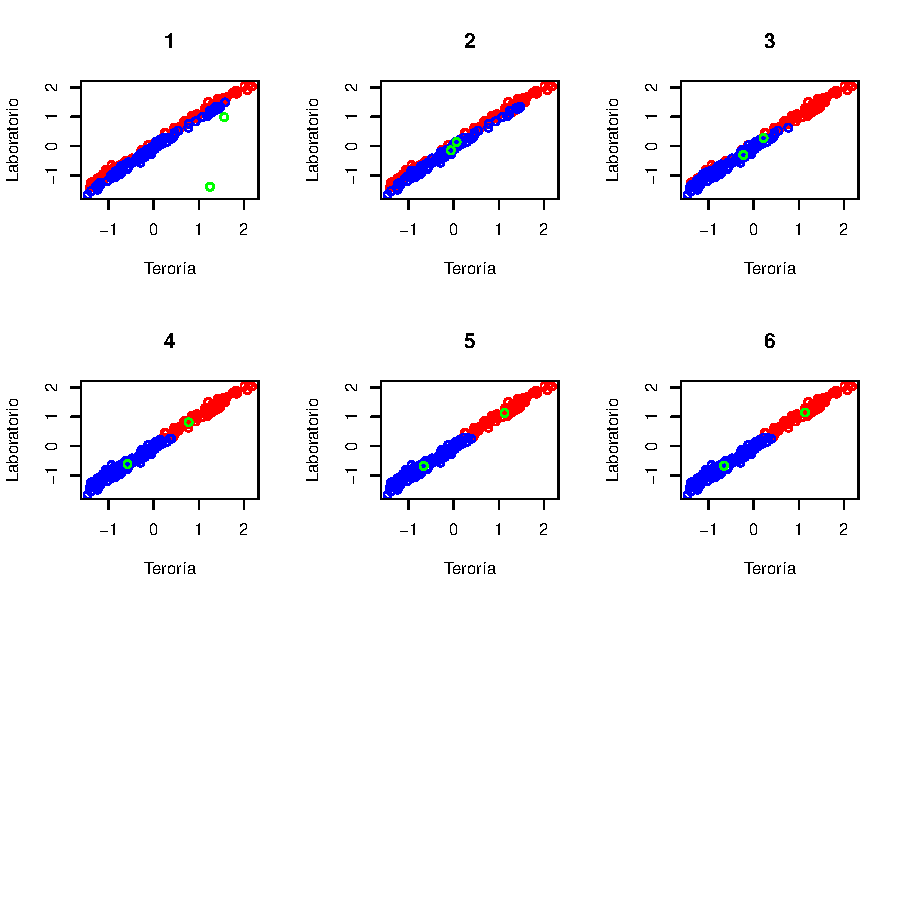
\includegraphics{entrega-kmeans_our_implementation}
\end{center}

Comprobamos adicionalmente que ambas clasificaciones, la de R y la nuestara coinciden como método de validación de nuestro algoritmo.
El porcentaje de similitud entre ambas clasificaciones oscila entre el 96\% y el 99\%.
El resultado es positivo.
\begin{Schunk}
\begin{Sinput}
> clusters <- cbind(k2$cluster,datos)
> cluster1 <- subset(clusters,clusters[,1]==1)
> cluster2 <- subset(clusters,clusters[,1]==2)
> cluster1 <- cluster1[,-1]
> cluster2 <- cluster2[,-1]
> clusters <- list(cluster1, cluster2)
> compare_clusters(clusters, split)
\end{Sinput}
\begin{Soutput}
[1] 0.9857143
\end{Soutput}
\end{Schunk}
Para que esta comparativa tenga algo de fiabilidad buscamos la mayor de las coincidencias entre las combinaciones válidas de las clasificaciones proporcionados por ambos métodos.
Debido a las componentes aleatorias de este algoritmo puede que a cada ejecución se produzcan resultados distintos.
Estos resultados cambiarán la posición de los centroides obtenidos pudiendo ser el centroide que antes era el representante de unos datos ser el representate de otros.
Por ello buscamos que combinación de asignaciones de centroides maximiza la similitud entre las clasificaciones.

\newpage
\subsection{Elección del número de clusters}
Hasta ahora hemos elegido siempre 2 como el número de clusters.
No obstante esta decisión no debiera ser trivial.
Expondremos a continuación una serie de métodos que pueden guiarnos a la hora de tomar esta decisión.

\subsubsection{Elbow Method}
Este método se basa en calcular la suma de las distancias cuadráticas medias entre los elementos de los clusters y dibujarlas en una gráfica.
Este valor es el proporcionado en "tot.withinss" al ejecutar kmeans tal y como ya explicamos en el primer apartado.
En la gráfica el número de cluster óptimos será aquel en el que se produzca un codo en la gráfica.
La suma de las distancias se irá reduciendo hasta llegar a 0 cuando haya tantas clases como elementos.
El punto de nuestro interés está en el momento en el que la gráfica comienza a descender a un ritmo menor.
\begin{center}
\begin{Schunk}
\begin{Sinput}
> wss <- function(k) {
+   kmeans(df, k, nstart = 10 )$tot.withinss
+ }
> k.values <- 1:15
> wss_values <- map_dbl(k.values, wss)
> plot(k.values, wss_values,
+        type="b", pch = 19, frame = FALSE, 
+        xlab="Number of clusters K",
+        ylab="Total within-clusters sum of squares")
\end{Sinput}
\end{Schunk}
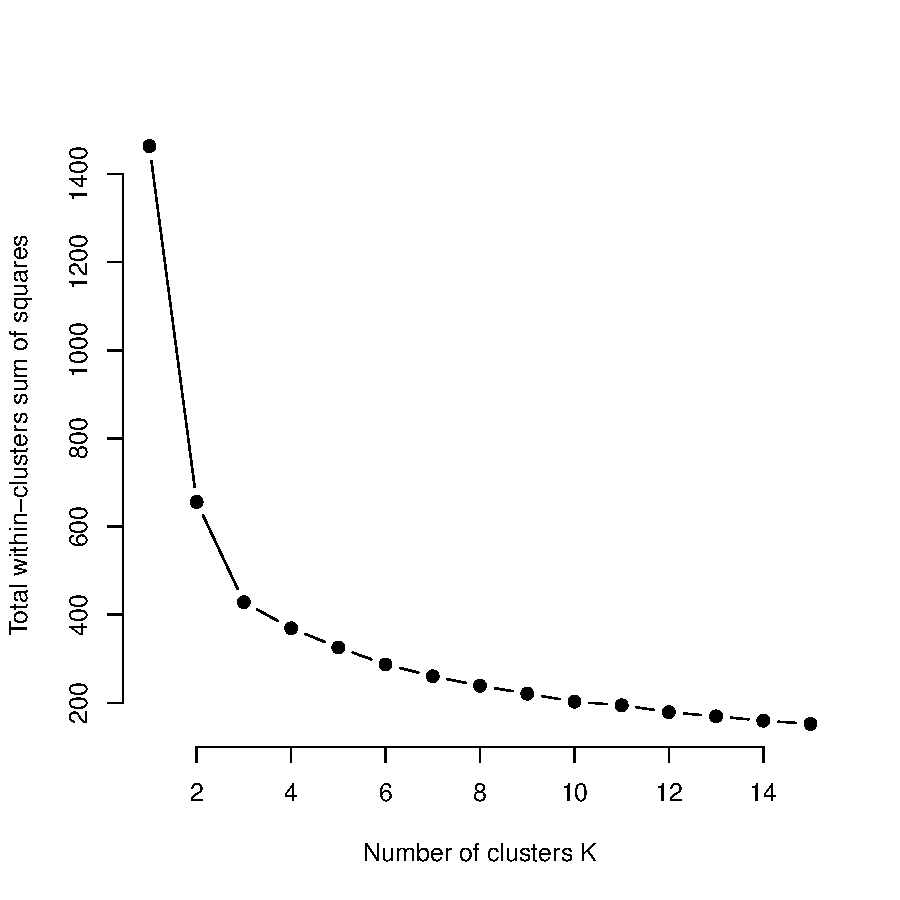
\includegraphics{entrega-optimal_number_of_clusters_1}
\end{center}
La siguiente función ya implementa este método de modo que no es necesario realizarlo manualmente.
\begin{center}
\begin{Schunk}
\begin{Sinput}
> fviz_nbclust(df, kmeans, method = "wss")
\end{Sinput}
\end{Schunk}
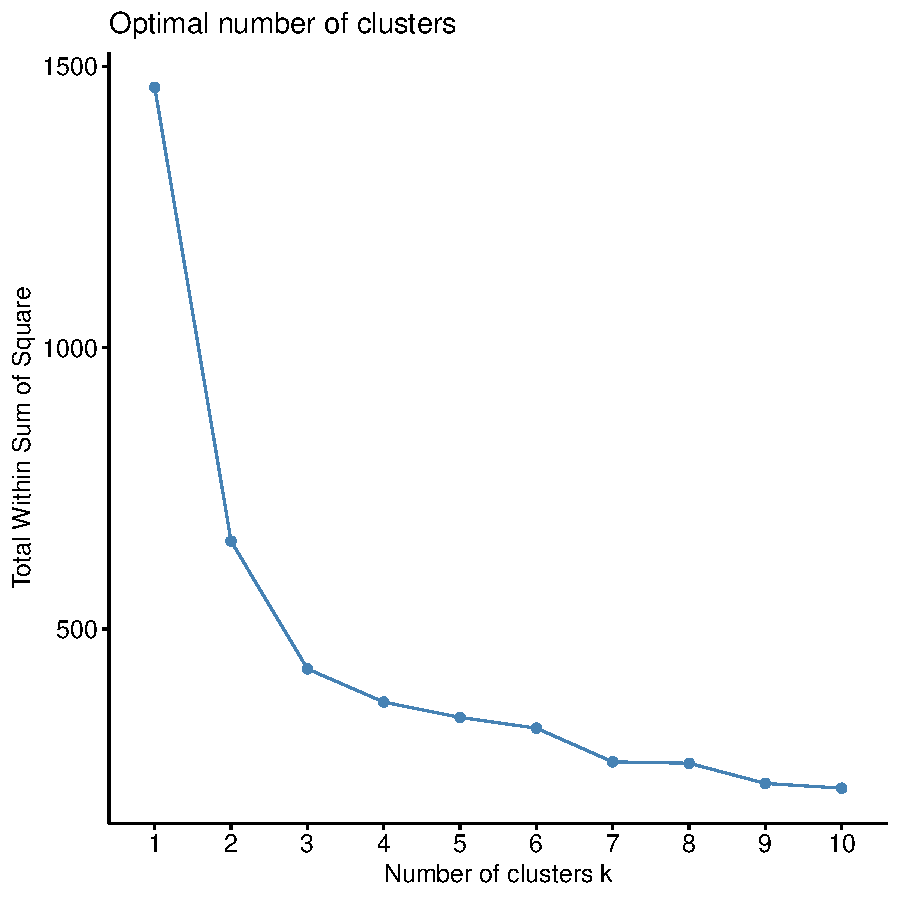
\includegraphics{entrega-optimal_number_of_clusters_2}
\end{center}

Podemos ver que el número de clusters óptimo estaría entre los valores de 2 y 4 clases.

\subsubsection{Average Silhouette Method}
Este método trata de calcular la paertenencia de cada elemento al cluster en el que ha sido clasificado.
Lo calcularemos manualmente para los valores de 2 a 15 clases.
Buscamos en esta gráfica aquellos números de clusters que maximizan la pertencencia de sus elementos.
\begin{center}
\begin{Schunk}
\begin{Sinput}
> avg_sil <- function(k) {
+   km.res <- kmeans(df, centers = k, nstart = 25)
+   ss <- silhouette(km.res$cluster, dist(df))
+   mean(ss[, 3])
+ }
> k.values <- 2:15
> avg_sil_values <- map_dbl(k.values, avg_sil)
> plot(k.values, avg_sil_values,
+        type = "b", pch = 19, frame = FALSE, 
+        xlab = "Number of clusters K",
+        ylab = "Average Silhouettes")
\end{Sinput}
\end{Schunk}
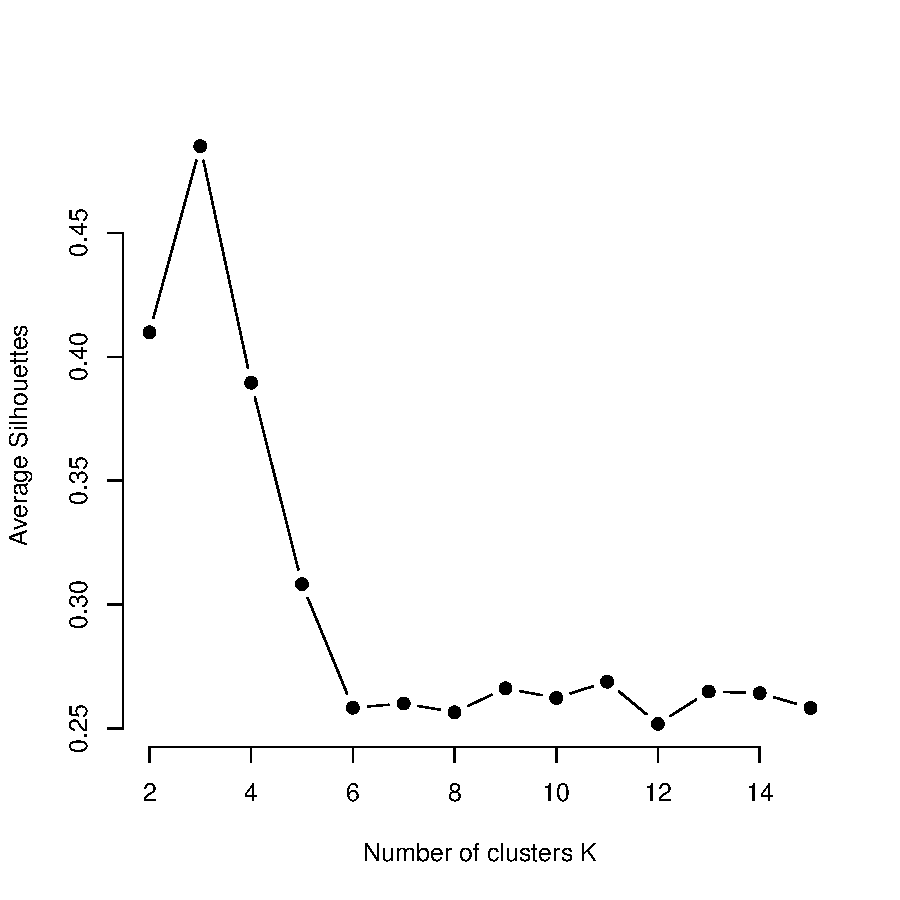
\includegraphics{entrega-optimal_number_of_clusters_3}
\end{center}
El mismo método está ya implementado en una única función.
\begin{center}
\begin{Schunk}
\begin{Sinput}
> fviz_nbclust(df, kmeans, method = "silhouette")
\end{Sinput}
\end{Schunk}
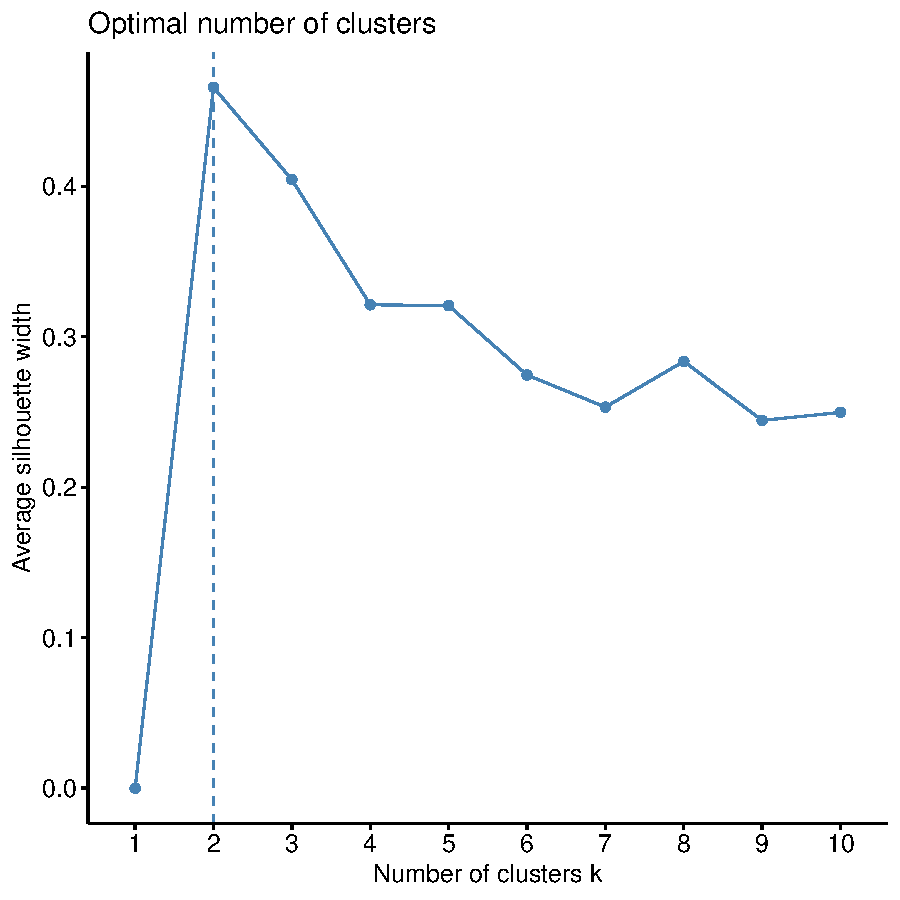
\includegraphics{entrega-optimal_number_of_clusters_4}
\end{center}

Podemos ver que 2 clases tiene la mayor pertenencia de los elementos clasificados a los clusters seguido de 3 clases.
Estos valores coinciden con los obtenidos con el método anterior.

\subsubsection{Gap Statistic Method}
Este es un método más complejo que los anteriores. La explicación del mismo puede verse en: http://web.stanford.edu/~hastie/Papers/gap.pdf.
Como resultados se obtiene una gráfica cuyo valor más alto será el mejor número de clusters.
Junto a cada valor se nos indica la calidad de la estimación.
Buscamos la combinación de un valor más alto en la gráfica con unos bigotes de menor tamaño.
\begin{center}
\begin{Schunk}
\begin{Sinput}
> gap_stat <- clusGap(df, FUN = kmeans, nstart = 25, K.max = 10, B = 50, verbose=FALSE)
> fviz_gap_stat(gap_stat)
\end{Sinput}
\end{Schunk}
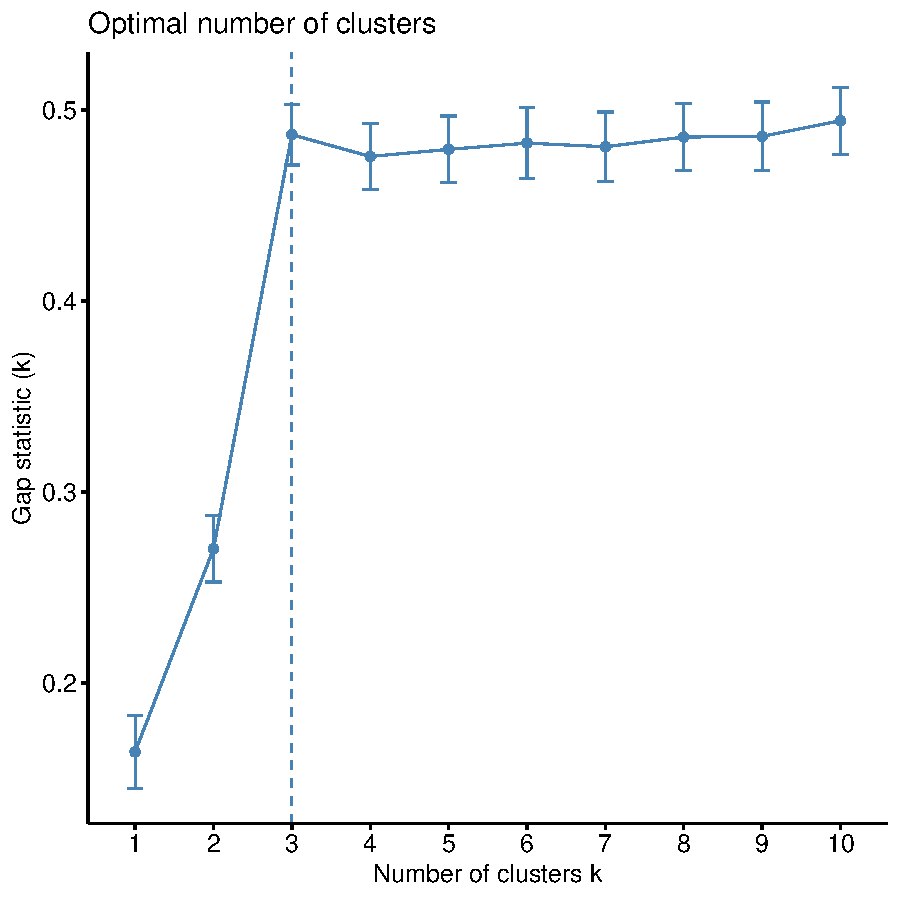
\includegraphics{entrega-optimal_number_of_clusters_5}
\end{center}

Podemos ver que en este caso 3 sería el mejor número de cluster en los que realizar nuestra clasificación.

Mostramos a continuación las distintas clasificciones que se obtienen cuando tenemos de 2 a 5 clases.
\begin{center}
\begin{Schunk}
\begin{Sinput}
> k3 <- kmeans(df, centers = 3, nstart = 25)
> k4 <- kmeans(df, centers = 4, nstart = 25)
> k5 <- kmeans(df, centers = 5, nstart = 25)
> p1 <- fviz_cluster(k2, geom = "point", data = df) + ggtitle("k = 2")
> p2 <- fviz_cluster(k3, geom = "point",  data = df) + ggtitle("k = 3")
> p3 <- fviz_cluster(k4, geom = "point",  data = df) + ggtitle("k = 4")
> p4 <- fviz_cluster(k5, geom = "point",  data = df) + ggtitle("k = 5")
> grid.arrange(p1, p2, p3, p4, nrow = 2)
\end{Sinput}
\end{Schunk}
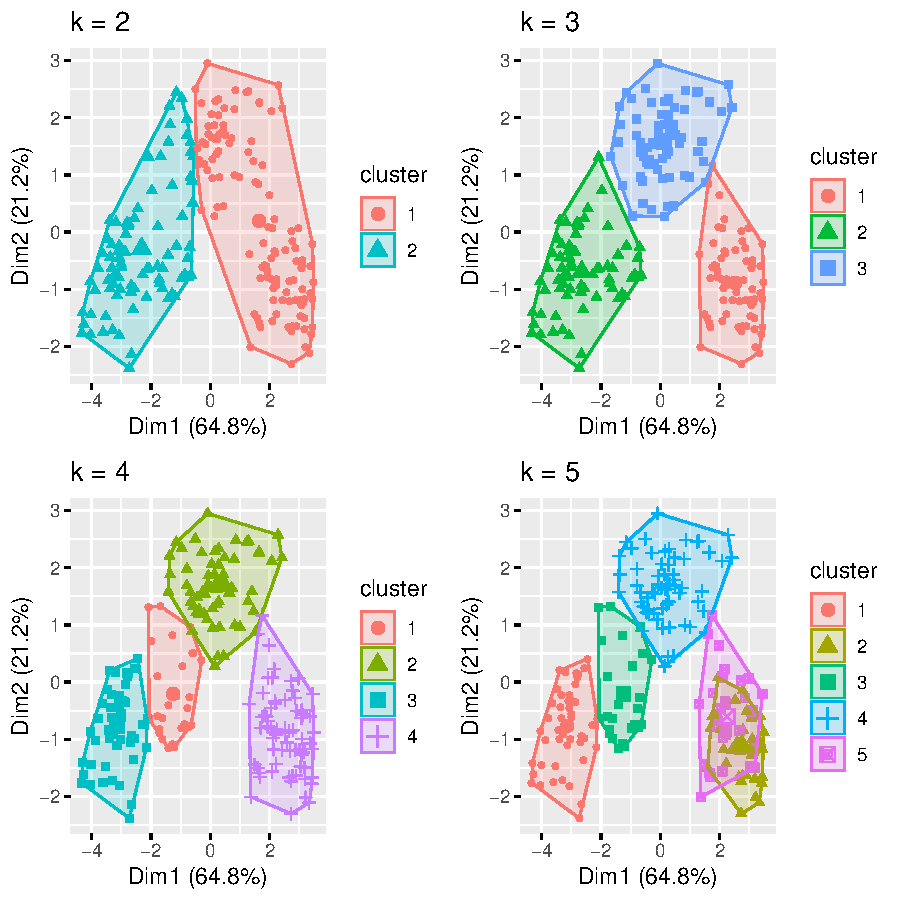
\includegraphics{entrega-kmeans_different_number_of_clusters}
\end{center}

Finalmente mostramos la suma de las distancias entre los elementos de los clusters y entre los clusters.
Vemos como al aumentar el número de clusters la calidad de la clasificación dentro de los clusters aumenta mientra que la calidad de la clasificación entre cluster disminuye.
Es por tanto que la elección del número de cluster es una optimización de estas dos variables teniendo en cuenta que puede que nos interese favorecer a una frente a la otra.
\begin{Schunk}
\begin{Sinput}
> c(k2$betweens, k3$betweens, k4$betweens, k5$betweens)
\end{Sinput}
\begin{Soutput}
[1]  806.9672 1034.3918 1093.5829 1138.0440
\end{Soutput}
\begin{Sinput}
> c(k2$tot.withinss, k3$tot.withinss, k4$tot.withinss, k5$tot.withinss)
\end{Sinput}
\begin{Soutput}
[1] 656.0328 428.6082 369.4171 324.9560
\end{Soutput}
\end{Schunk}

\newpage
\section{Clusterización jerárquica}
Utilizaremos y compararemos los método de clusterización ascendente y descendente.
Adicionalmente en la clusterización jerárquica ascendente compararemos distintas medidas de distancia por las que se juntan los clusters.
Adicionalmente compararemos los resultados obtenidos con los obtenidos en k-means.
Para hacerlo utilizaremos 3 como número de clusters en los que clasificar ya que como vimos en apartados anteriores este era un número adecuado de clusters en los que dividir la muestra.
Utilizaremos funciones de las siguiente librerías: "cluster", "purrr", "dendextend" y "factoextra".

\subsection{Preparar los datos}
Al igual que hicimos en el apartado anterior comenazaremos por preparar los datos eliminando los elementos nulos y escalándolos.
El escalado deja los datos con media 0 y desviación estándar de 1.
\begin{Schunk}
\begin{Sinput}
> data <- read.csv("Seed_Data.csv")
> data <- na.omit(data)
> data <- scale(data)
\end{Sinput}
\end{Schunk}

\subsection{Clusterización jerárquica ascendente}
En esta clusterización partiremos de que cada dato de la muestra es su propio cluster de modo que los iremos agrupando según distintas métricas hasta formar un único cluster.
Para clasificar por otro número de cluster solo deberemos descender en el árbol creado hasta el nivel de división adecuado.

Para poder realizar la clusterización jerárquica ascendente necesitamos calcular las distancias entre los elementos.
Dichas distancias serán utilizadas por el algoritmo de clusterización para realizar la clasificación no supervisada.
Utilizaremos la distancia euclídea para calcular la distancia entre los puntos.
Tal y como vivmos en clase solo es necesario calcular la distancia entre los puntos una sola vez,
posteriormente dependiendo del método utilizado la matriz de distancias se actualizará con la distancia máxima, mínima o media de los clusters que se unan.
\begin{Schunk}
\begin{Sinput}
> d <- dist(data, method = "euclidean")
\end{Sinput}
\end{Schunk}

\subsubsection{Clusterización jerárquica ascendente complete-linkage}
Mediante este método las actualizaciones de la matriz de distancias se realizarán con el operador max.
Es decir, cuando unamos dos clusters entre si, la distancia del nuevo cluster al resto de puntos será la distancia máxima de cada uno de esos puntos a todos los del cluster.
\begin{center}
\begin{Schunk}
\begin{Sinput}
> jerarquica_acendente_completa <- hclust(d, method = "complete")
> plot(jerarquica_acendente_completa, cex = 0.6, hang = -1)
> rect.hclust(jerarquica_acendente_completa, k = 3, border = 2:10)
\end{Sinput}
\end{Schunk}
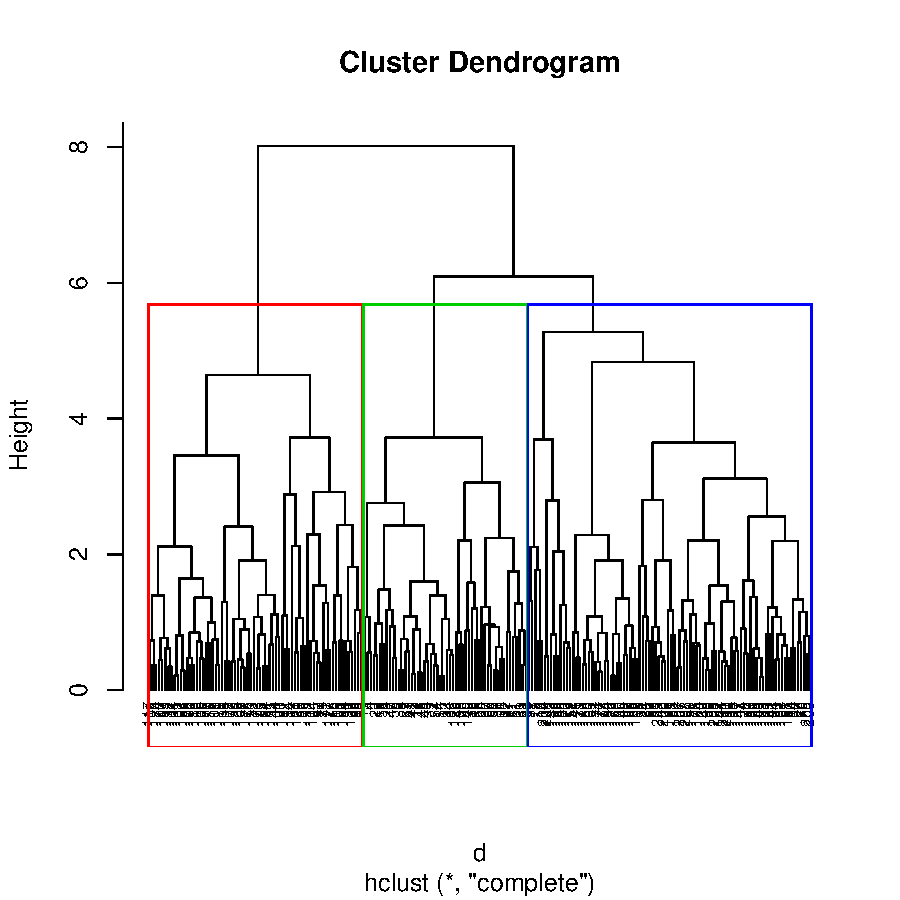
\includegraphics{entrega-jerarquica_acendente_completa}
Vemos que aproximadamente cada clase toma un tercio de los datos.
Adicionalmete la proyección de la representación visual nos da a entender que los clusters separan de forma adecuada a la muestra.
Esto que ahora solo podemos estimar de la visualización lo exploraremos numéricamente más adelante.
\begin{Schunk}
\begin{Sinput}
> jerarquica_acendente_completa_clust <- cutree(jerarquica_acendente_completa, k = 3)
> fviz_cluster(list(data = data, cluster = jerarquica_acendente_completa_clust))
\end{Sinput}
\end{Schunk}

\includegraphics{entrega-jerarquica_acendente_completa_plot}
\end{center}

\subsubsection{Clusterización jerárquica ascendente average-linkage}
Cuando unamos dos clusters actualizaremos la matriz de distancias con el operador media aritmética.
La nueva distancia del cluster al resto de ellos será la distancia media de sus puntos a cada uno de los de cada otro cluster.
\begin{center}
Al igual que con complete-linkage podemos ver que cada clase tiene aproximadamente un tercio de los datos y que la clasificación separa adecuadamente a la muestra.
\begin{Schunk}
\begin{Sinput}
> jerarquica_acendente_media <- hclust(d, method = "average")
> plot(jerarquica_acendente_media, cex = 0.6, hang = -1)
> rect.hclust(jerarquica_acendente_media, k = 3, border = 2:10)
\end{Sinput}
\end{Schunk}
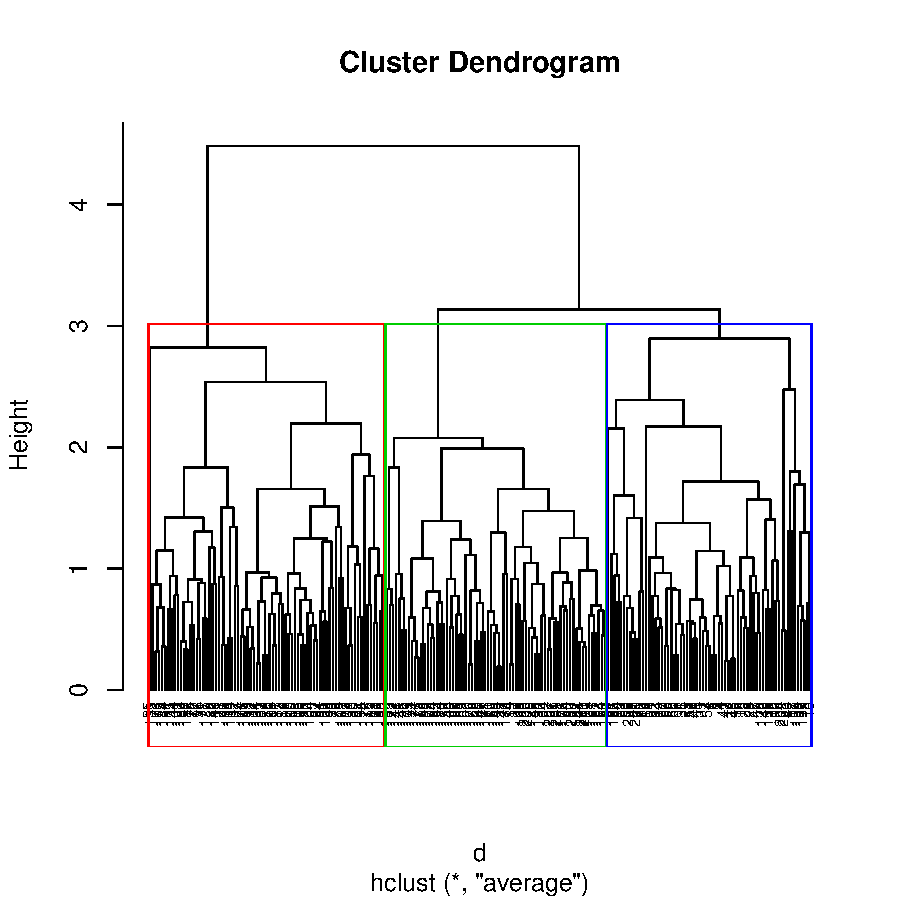
\includegraphics{entrega-jerarquica_acendente_media}
\begin{Schunk}
\begin{Sinput}
> jerarquica_acendente_media_clust <- cutree(jerarquica_acendente_media, k = 3)
> fviz_cluster(list(data = data, cluster = jerarquica_acendente_media_clust))
\end{Sinput}
\end{Schunk}
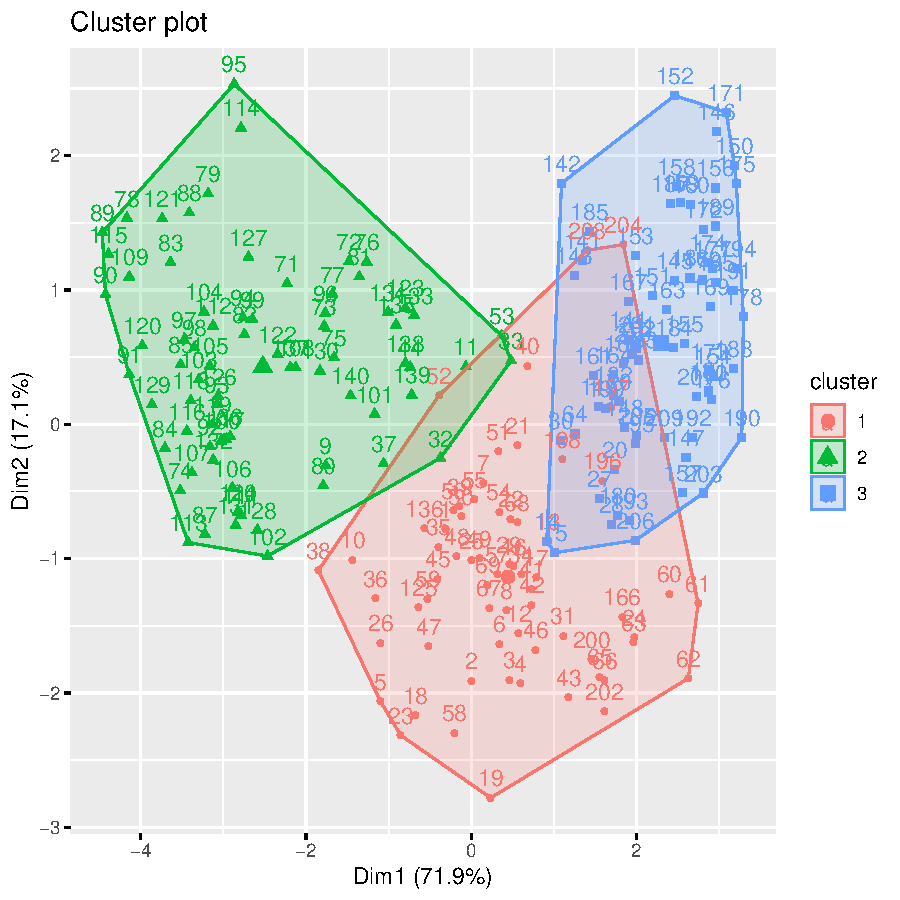
\includegraphics{entrega-jerarquica_acendente_media_plot}
\end{center}

\subsubsection{Clusterización jerárquica ascendente single-linkage}
La actualización de la matriz de distancias mediante este método se raliza mediante el operador mínimo.
Cuando dos cluster se unan la matriz se actualizará con la distancia mínima de los puntos del nuevo cluster a los puntos de cada uno de los otros clusters.
\begin{center}
\begin{Schunk}
\begin{Sinput}
> jerarquica_acendente_single <- hclust(d, method = "single")
> plot(jerarquica_acendente_single, cex = 0.6, hang = -1)
> rect.hclust(jerarquica_acendente_single, k = 3, border = 2:10)
\end{Sinput}
\end{Schunk}
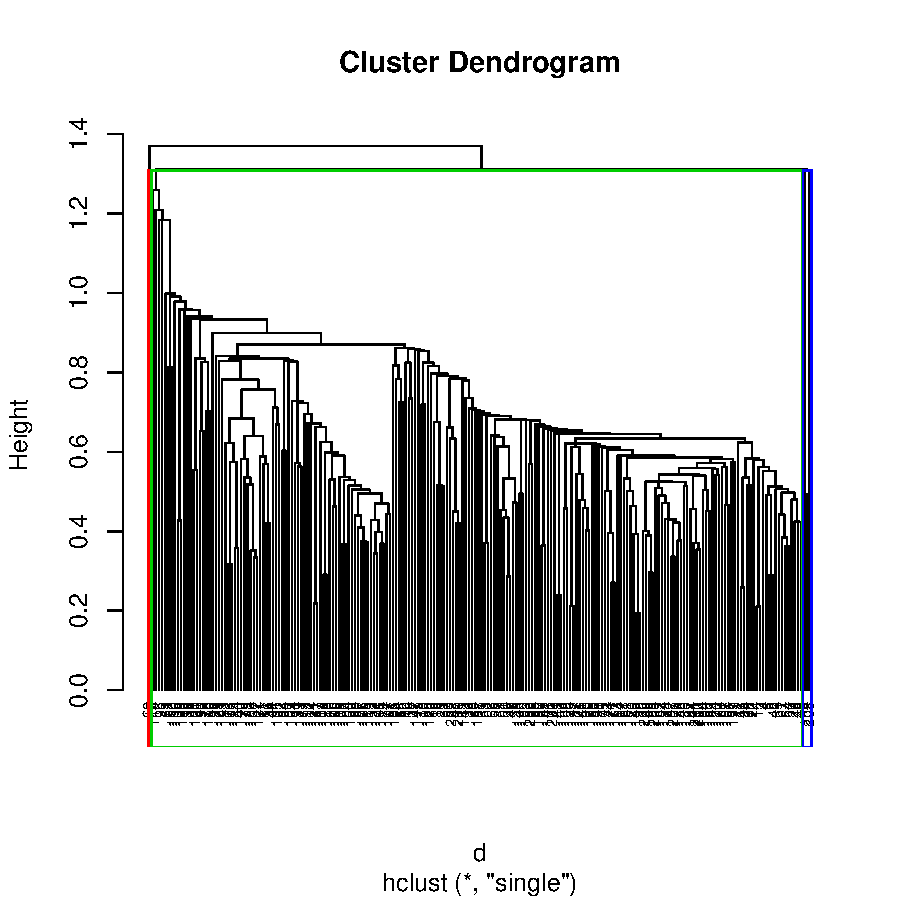
\includegraphics{entrega-jerarquica_acendente_single}
En este caso vemos como una única clase está asociada a la mayoría de los datos siendo las otras dos muy pequeñas.
Puede que esto se deba a que este método de clusterización jerárquica ascendente no deba ser utilizado así.
También puede que se deba por la estructura de los datos que haga que este método no sea adecuado para ellos.
\begin{Schunk}
\begin{Sinput}
> jerarquica_acendente_single_clust <- cutree(jerarquica_acendente_single, k = 3)
> fviz_cluster(list(data = data, cluster = jerarquica_acendente_single_clust))
\end{Sinput}
\end{Schunk}
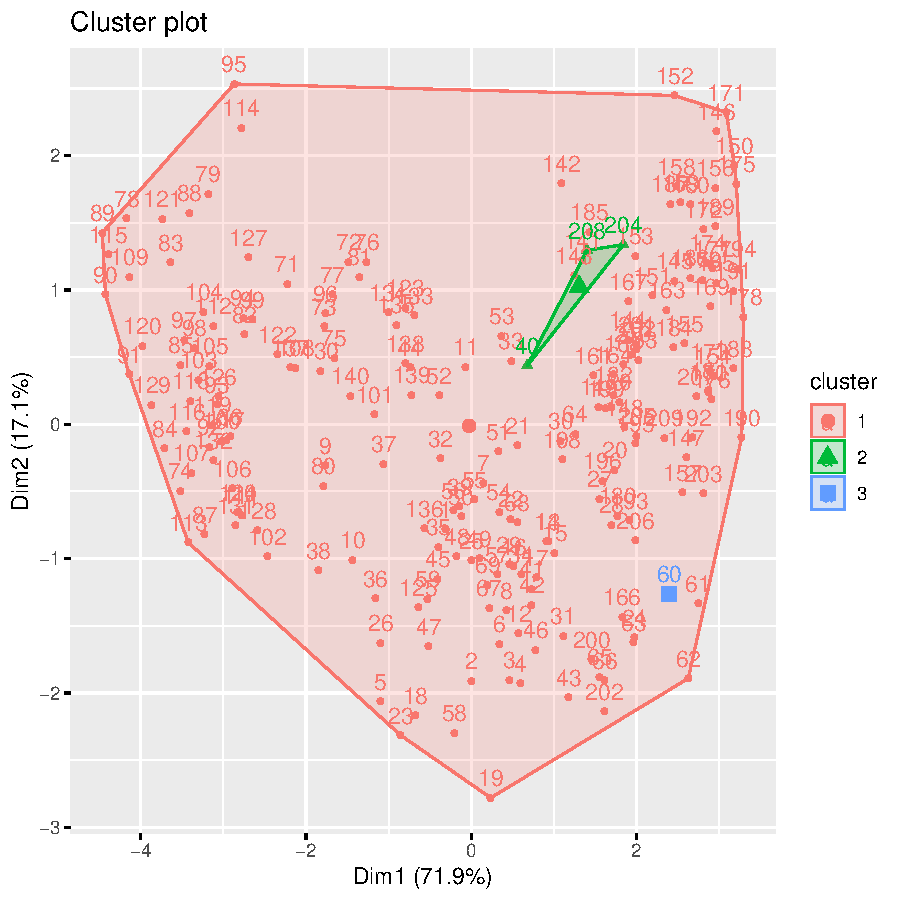
\includegraphics{entrega-jerarquica_acendente_single_plot}
\end{center}

\subsubsection{Clusterización jerárquica ascendente ward-linkage}
Este método es el más diferente comparado con los otros tres.
En este caso nos se juntarán dos cluster por que la distancia entre ellos sea la menor distancia de la matriz de distancias si no
porque su unión es la unión que produce una pérdida de información mínima.
\begin{center}
\begin{Schunk}
\begin{Sinput}
> jerarquica_acendente_ward <- hclust(d, method = "ward.D")
> plot(jerarquica_acendente_ward, cex = 0.6, hang = -1)
> rect.hclust(jerarquica_acendente_ward, k = 3, border = 2:10)
\end{Sinput}
\end{Schunk}
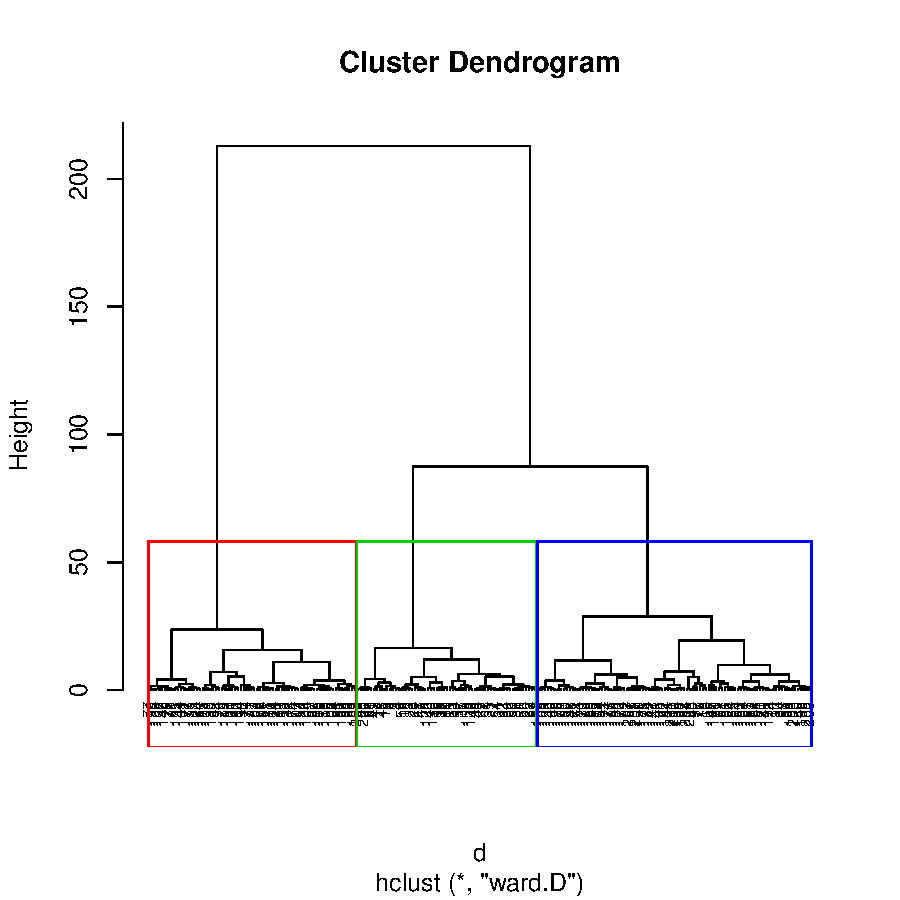
\includegraphics{entrega-jerarquica_acendente_ward}
Con este método las clases vuelven a ser de un tamaño próximo al tercio de la muestra y los clusters vuelven a parecer bastante separados.
\begin{Schunk}
\begin{Sinput}
> jerarquica_acendente_ward_clust <- cutree(jerarquica_acendente_ward, k = 3)
> fviz_cluster(list(data = data, cluster = jerarquica_acendente_ward_clust))
\end{Sinput}
\end{Schunk}
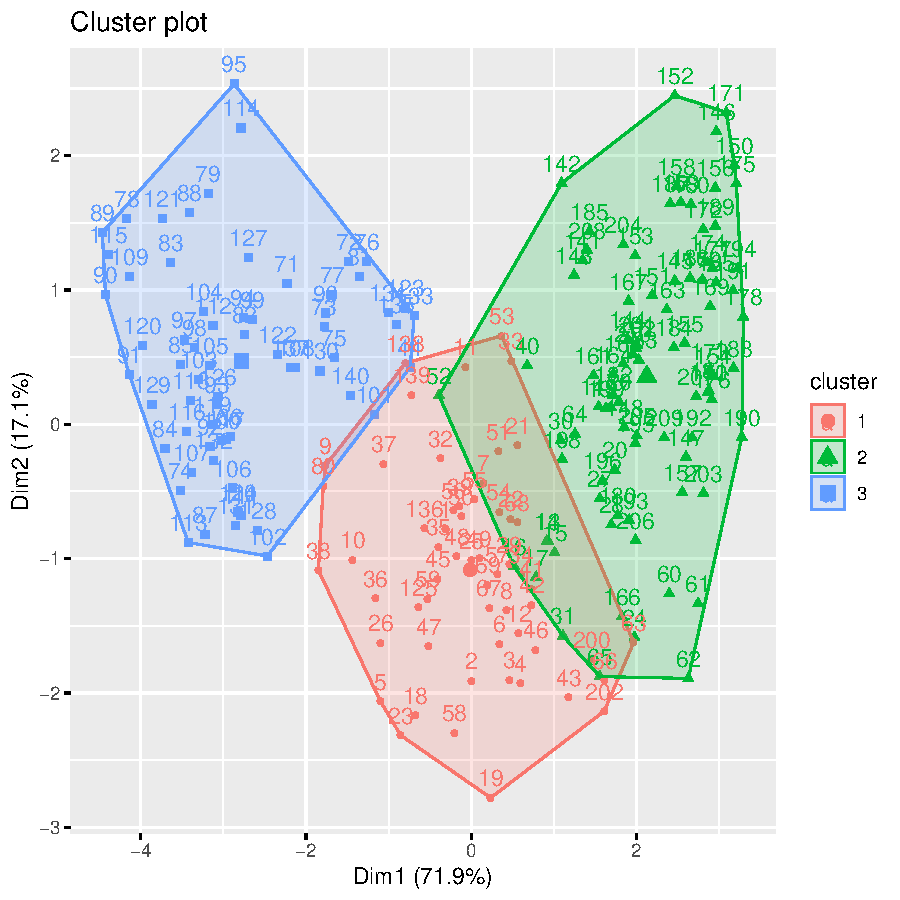
\includegraphics{entrega-jerarquica_acendente_ward_plot}
\end{center}

\subsubsection{Coeficiente aglomerativo}
Otra función con la que realizar la clasificación jerárquica ascendente es "agnes".
Los resultados obtendidos son los mismos que los que se obtienen con "cutree" ya que realizan las mismas operaciones.
Adicionalmente para dibujarlos se pueden seguir utilizando las mismas funciones.
La principal diferencia entre "agnes" y "cutree" es que la primera nos proporciona el coeficiente aglomerativo de los clusters generados.

Dicho coeficiente nos informa sobre lo buena o mala que a sido la clasificación a partir de indicarnos cómo de densos son los clusters generados.
Los valores de coeficiente aglomerativo próximos a 1 nos indican que la homogeneidad entre los elementos de los cluster es elevada.

Calcularemos dicho coeficiente para cada una de las medidas de agrupación de datos.
Deseamos que este número sea los más alto posible de modo que los clusters sean homogéneos dentro de ellos y heterogéneos entre si.
Como vemos los resultados de calcular el coeficiente no coincide con el análisis realizado sobre las gráficas y los dendogramas.

Ward obtiene el mayor coeficiente aglomerativo debido a que minimiza la pérdida de información con la cual este se relaciona.
Single sorprendentemente obtiene un buen coeficienter aglomerativo mientras que average no lo hace.
\begin{Schunk}
\begin{Sinput}
> methods <- c( "average", "single", "complete", "ward")
> names(methods) <- c("complete", "average", "single", "ward")
> aglomerative_coeficient <- function(method) {
+   agnes(data, method = method)$ac
+ }
> map_dbl(methods, aglomerative_coeficient)
\end{Sinput}
\begin{Soutput}
 complete   average    single      ward 
0.8649547 0.6055379 0.9231512 0.9846264 
\end{Soutput}
\end{Schunk}

\subsubsection{Comparación con kmeans}
Calculamos a continución el porcentaje de datos que fueron clasificados en las mismas clases que lo fueron en k-means.
Para ello utilizamos la misma función que ya utilizamos para comparar los resultados de nuestro k-menas con los del k-means implementado por R.
Podemos ver que complete-linkage y avergae-linkage producen las clasificaciones más similares a las de k-means.
Por el contrario en el caso de single está claro que este valor no iba a poder ser dmasiado elevado.
Sorprende que con ward el valor sea elevado ya que en la representación los cluster eran similares a los de k-means con k=3,
no obstante tal y como ya explicamos esa representación no es demasido fiable ya que pone en solo 2 dimensiones datos de 7 dimensiones.
\begin{Schunk}
\begin{Sinput}
> clusters_jerarquico_ascendente <- list( jerarquica_acendente_completa_clust,
+                                      jerarquica_acendente_media_clust, 
+                                      jerarquica_acendente_single_clust, 
+                                      jerarquica_acendente_ward_clust)
> names(clusters_jerarquico_ascendente) <- c("complete", "average", "single", "ward")
> kmeans_compare <- function(cluster) {
+   compare_clusters(clusters_kmeans, split_clusters(cluster))
+ }
> map_dbl(clusters_jerarquico_ascendente, kmeans_compare)
\end{Sinput}
\begin{Soutput}
 complete   average    single      ward 
0.8809524 0.8952381 0.3380952 0.3761905 
\end{Soutput}
\end{Schunk}

\newpage
\subsection{Clusterización jerárquica descendente}
La clasificación jerárquica descendente se realiza partiendo de un único cluster que comprende a todos los datos.
Poco a poco iremos descomponiendo este cluster en otros más pequeños hasta acabar con que cada dato esté en su propio cluster.
Para evaluar un número de cluster concreto actuaremos de forma similar a la clusterización jerárquica ascendente utilizando el árbol que se generados.

Clasificaremos la muestra con la función "diana".
\begin{center}
\begin{Schunk}
\begin{Sinput}
> jerarquico_descendente <- diana(data)
> pltree(jerarquico_descendente, cex = 0.6, hang = -1)
> rect.hclust(jerarquico_descendente, k = 3, border = 2:10)
\end{Sinput}
\end{Schunk}
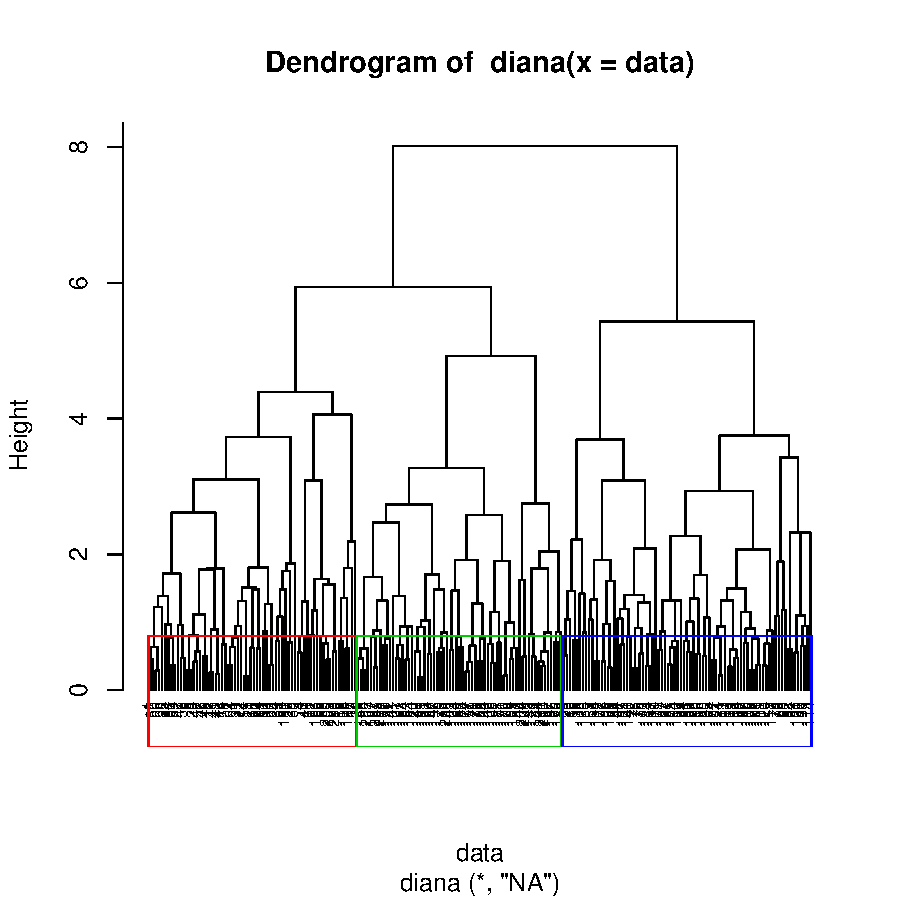
\includegraphics{entrega-jerarquico_descendente}
\end{center}
Podemos ver que cada clase contiene cerca de un tercio de los datos y que los cluster parecen separados entre si.
\begin{center}
\begin{Schunk}
\begin{Sinput}
> jerarquico_descendente_clust <- cutree(jerarquico_descendente, k = 3)
> fviz_cluster(list(data = data, cluster = jerarquico_descendente_clust))
\end{Sinput}
\end{Schunk}
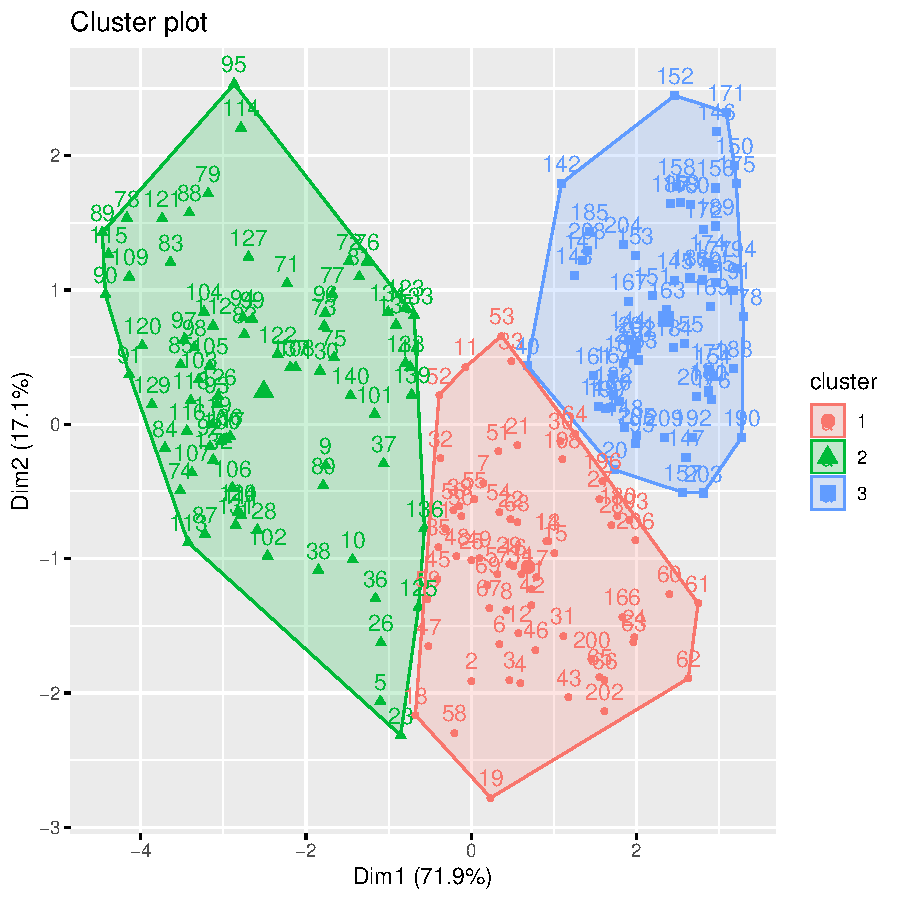
\includegraphics{entrega-jerarquico_descendente_plot}
\end{center}

\subsubsection{Coeficiente divisivo}
En este caso podremos medir la buena clasificación del algoritmo con el coeficiente divisivo que deseamos sea próximo a 1.
Este valor mide lo heterogéneos que son los cluster generados entre sí.
\begin{Schunk}
\begin{Sinput}
> jerarquico_descendente$dc
\end{Sinput}
\begin{Soutput}
[1] 0.918148
\end{Soutput}
\end{Schunk}

\subsubsection{Comparación con kmeans}
Este método produce una clasificación muy similar a la de k-means, el 90\% de los valores han sido calsificados del mismo modo.
\begin{Schunk}
\begin{Sinput}
> compare_clusters(clusters_kmeans, split_clusters(jerarquico_descendente_clust))
\end{Sinput}
\begin{Soutput}
[1] 0.9
\end{Soutput}
\end{Schunk}

\newpage
\subsection{Comparación de dendogramas}
Finalmente mostraremos el uso de la función "tanglegram" que toma como entrada dos dendogramas.
Como 
\begin{center}
\begin{Schunk}
\begin{Sinput}
> hc_single <- agnes(data, method = "average")
> hc_complete <- agnes(data, method = "ward")
> hc_single <- as.dendrogram(hc_single)
> hc_complete <- as.dendrogram(hc_complete)
> tanglegram(hc_single,hc_complete)
\end{Sinput}
\end{Schunk}
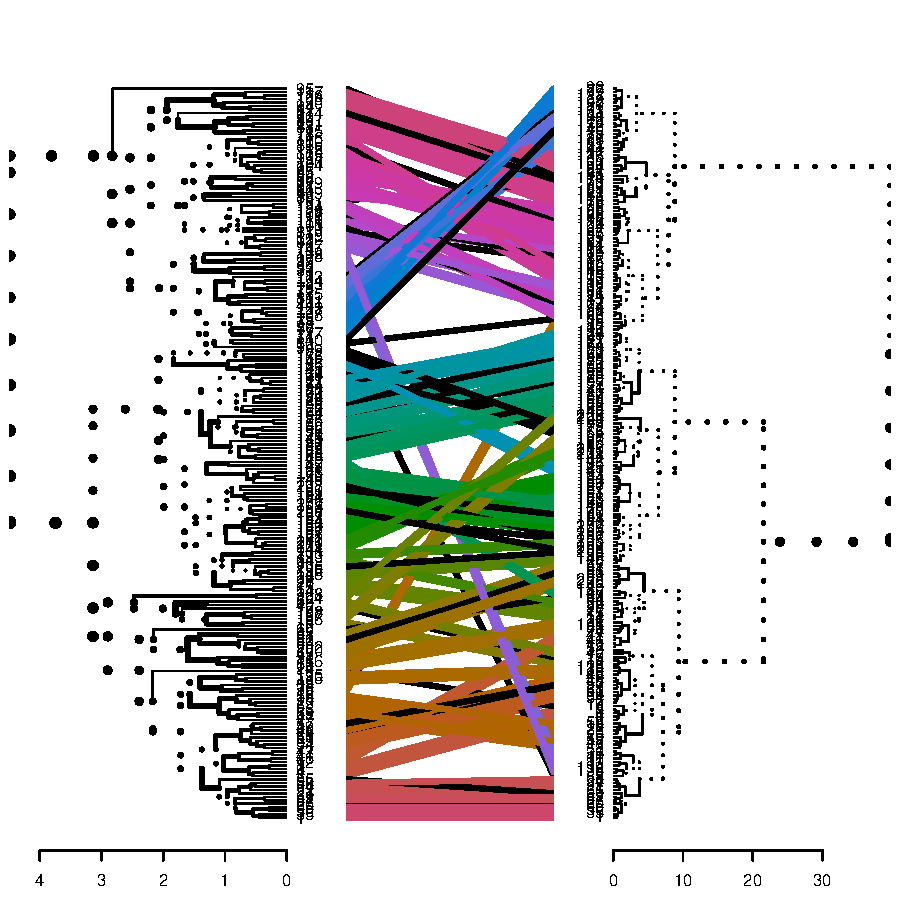
\includegraphics{entrega-jerarquico_comparacion_dendogramas}
\end{center}

\newpage
\section{Funciones implementadas}
Las funcines creadas son las que implementan k-means así como una función adicional para crear las gráficas con los resultados.
\subsection{distance}
Nos da la distancia euclídea entre dos puntos.
\begin{Schunk}
\begin{Sinput}
> distance
\end{Sinput}
\begin{Soutput}
function (point1, point2) {
  acc <- 0
  len <- length(point1)
  for (i in 1:len){
    acc <- acc + (point1[i]-point2[i])^2
  }
  acc^(1/2)
}
<bytecode: 0x7fbf9adba230>
\end{Soutput}
\end{Schunk}
\subsection{kmeans cluster}
Indica la pertenencia de los elementos de la muestra a las clases marcadas por los centroides.
\begin{Schunk}
\begin{Sinput}
> kmeans_cluster
\end{Sinput}
\begin{Soutput}
function (data, centroids) {
  d_default <- distance(c(max(data), max(data)), c(min(data), min(data)))
  classification <- c()
  for (j in 1:nrow(data)){
      point <- data[j,]
      best_c <- 0
      best_d <- d_default
      for (i in 1:nrow(centroids)){
        centroid <- centroids[i,]
        d <- distance (point, centroid)
        if (d < best_d){
          best_d <- d
          best_c <- i
        }
    }
    classification <- c(classification, best_c)
  }
  classification <- as.data.frame(classification)
  rownames(classification) <- rownames(data)
  classification
}
<bytecode: 0x7fbf9bb2dd08>
\end{Soutput}
\end{Schunk}
\subsection{kmeans split}
Crea una lista cuyos elementos son conjuntos de elemenyos del mismo cluster.
\begin{Schunk}
\begin{Sinput}
> kmeans_split
\end{Sinput}
\begin{Soutput}
function (data, cluster) {
  clusters=cbind(cluster,data)
  cluster1=subset(clusters,clusters[,1]==1)
  cluster2=subset(clusters,clusters[,1]==2)
  cluster1=cluster1[,-1]
  cluster2=cluster2[,-1]
  list(cluster1, cluster2)
}
<bytecode: 0x7fbf9ea503a0>
\end{Soutput}
\end{Schunk}
\subsection{kmeans new centroids}
Crea nuevos centroides a partir de la distancia media de cada uno de ellos a los elementos de su clase.
\begin{Schunk}
\begin{Sinput}
> kmeans_new_centroids
\end{Sinput}
\begin{Soutput}
function(split){
  centroids <- c()
  for (cluster in split) {
    for (colum in cluster) {
      acc <- 0
      for (element in colum){
        acc <- acc + element/length(colum)
      }
      centroids <- c(centroids, acc)
    }
  }
  t(matrix(centroids,length(split[[1]]),length(split)))
}
<bytecode: 0x7fbfa0271a28>
\end{Soutput}
\end{Schunk}
\subsection{same centroids}
Compara dos centroides para saber si son iguales.
\begin{Schunk}
\begin{Sinput}
> same_centroids
\end{Sinput}
\begin{Soutput}
function(c1, c2){
  len <- length(c1)
  ans <- T
  for (i in 1:len){
    if (c1[i]!=c2[i]){
      ans <- F
    }
  }
  ans
}
<bytecode: 0x7fbfa0187d08>
\end{Soutput}
\end{Schunk}
\subsection{plot kmeans}
Dibuja el resultado de una clasificación.
\begin{Schunk}
\begin{Sinput}
> plot_kmeans
\end{Sinput}
\begin{Soutput}
function (clusters, centers, main="", xlab="", ylab="") {
  maxx <- max(clusters[[1]][,1])
  maxy <- max(clusters[[1]][,2])
  minx <- min(clusters[[1]][,1])
  miny <- min(clusters[[1]][,2])
  for (cluster in clusters){
    maxx <- max(maxx, max(cluster[,1]))
    maxy <- max(maxy, max(cluster[,2]))
    minx <- min(minx, min(cluster[,1]))
    miny <- min(miny, min(cluster[,2]))
  }
  color_i <- 1
  colors = c("red", "blue", "pink", "yellow", "black", "brown")
  for (cluster in clusters){
    plot( cluster[,1], cluster[,2], type="p", col=colors[color_i],main=main,
          xlim=c(minx, maxx), ylim=c(miny, maxy), xlab=xlab, ylab=ylab)
    par(new=TRUE)
    color_i <- (color_i%%(length(colors)+1))+1
  }
  plot( centers[,1], centers[,2], type="p", col="green",
        xlim=c(minx, maxx), ylim=c(miny, maxy), xlab=xlab, ylab=ylab)
}
<bytecode: 0x7fbf9fcd2708>
\end{Soutput}
\end{Schunk}
\subsection{compare clusters}
Calcula el porcentaje de elementos comunes en dos clasificaciones distintas.
\begin{Schunk}
\begin{Sinput}
> compare_clusters
\end{Sinput}
\begin{Soutput}
function(c1, c2) {
  len <- length(c1)
  number_of_elements <- 0
  for (i in 1:len) {
    number_of_elements <- number_of_elements + nrow(c1[[i]])
  }
  same <- 0
  for (j in 1:len){
    current_same <- 0
    for (i in 1:len){
      r1 <- c1[[i]]
      r2 <- c2[[((i+j)%%len)+1]]
      r1_names <- rownames(r1)
      if (length(r1_names)<1){
        r1_names <- names(r1)
      }
      r2_names <- rownames(r2)
      if (length(r2_names)<1){
        r2_names <- names(r2)
      }
      if (length(r1_names) < length(r2_names)){
        temp <- r1_names
        r1_names <- r2_names
        r2_names <- temp
      }
      for (name in r1_names){
        if (name %in% r2_names){
          current_same <- current_same+1
        }
      }
    }
    same <- max(same, current_same)
  }
  same/number_of_elements
}
<bytecode: 0x7fbf9bb68910>
\end{Soutput}
\end{Schunk}

\end{document}
